\documentclass[border=10pt,12pt]{article}
\usepackage[a4paper,margin=2cm,landscape]{geometry}
\usepackage{pgfplots}
\pgfplotsset{compat=1.17}
\pagestyle{empty}

\begin{document}
\noindent
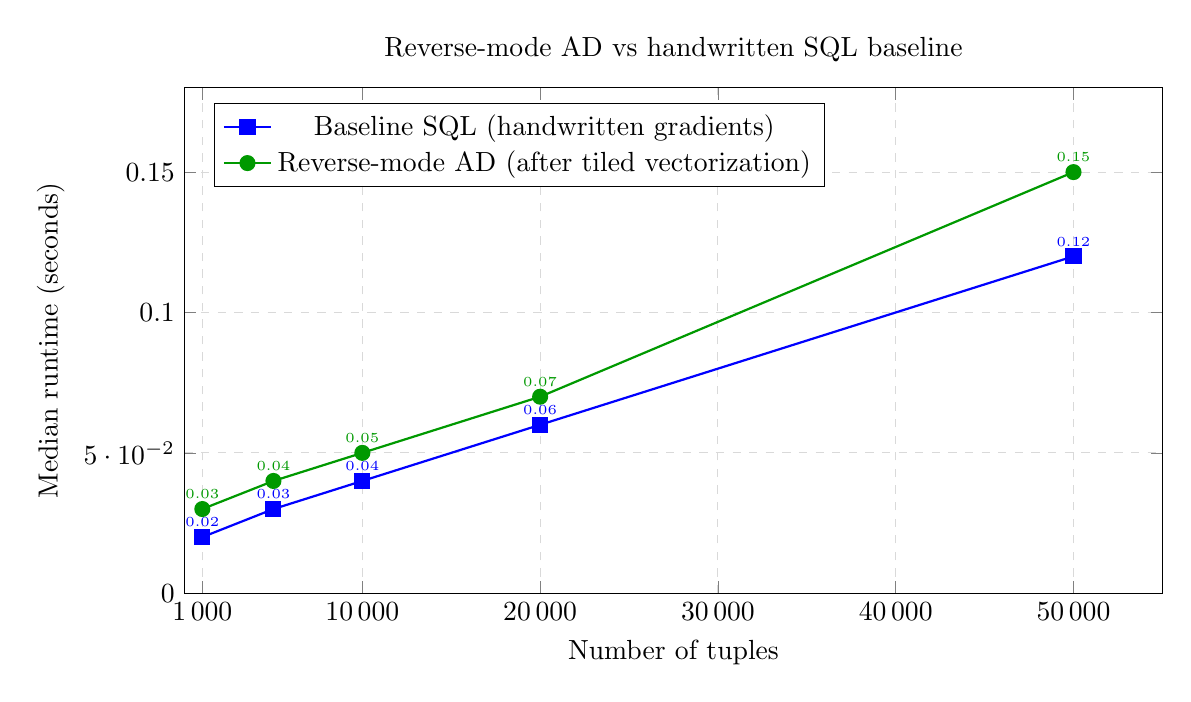
\begin{tikzpicture}
\begin{axis}[
    width=14cm,
    height=8cm,
    title={Reverse-mode AD vs handwritten SQL baseline},
    xlabel={Number of tuples},
    ylabel={Median runtime (seconds)},
    xmin=0, xmax=55000,
    ymin=0, ymax=0.18,
    xtick={1000,10000,20000,30000,40000,50000},
    scaled x ticks=false,
    xticklabel style={/pgf/number format/1000 sep=\,},
    legend pos=north west,
    grid=major,
    grid style={dashed,gray!30},
    nodes near coords,
    nodes near coords style={font=\tiny, anchor=south},
    point meta=explicit symbolic,
]

\addplot[color=blue, mark=square*, thick, mark size=2.5pt] coordinates {
    (1000, 0.02) [0.02]
    (5000, 0.03) [0.03]
    (10000, 0.04) [0.04]
    (20000, 0.06) [0.06]
    (50000, 0.12) [0.12]
};
\addlegendentry{Baseline SQL (handwritten gradients)}

\addplot[color=green!60!black, mark=*, thick, mark size=2.5pt] coordinates {
    (1000, 0.03) [0.03]
    (5000, 0.04) [0.04]
    (10000, 0.05) [0.05]
    (20000, 0.07) [0.07]
    (50000, 0.15) [0.15]
};
\addlegendentry{Reverse-mode AD (after tiled vectorization)}

\end{axis}
\end{tikzpicture}
\end{document}
